\clearpage
\scanpage{9}
\noindent\hfill\begin{tabular}{|c}Notations\\\hline\end{tabular}

\diagram{\resizebox{\linewidth}{!}{\(\displaystyle\begin{array}{@{}l|c@{}}
\underline{\underline{\mathrm{Quot}}}_{F/{\unsure{x|X}}/S}(S')=\Gamma(S',\underline{\mathrm{Quot}}(F'/X'/S'))=\mathrm{Quot}(F'/X'/S') & F\\[.5em]
\underline{\underline{\mathrm{Hilb}}}_{X/S}(S')=\Gamma(S',\underline{\mathrm{Hilb}}(X'/S'))=\mathrm{Hilb}(X'/S')\qquad-\qquad=\underline{\underline{\mathrm{Quot}}}_{\underline O_X/X/S}(S') & X\\[-.3em]
\quad\unsure{\prime} & \\[-.2em]
\underline{\underline{\mathrm{Div}\deleted{\mathrm{eff}}}}_{X/S}(S')=\Gamma(S',\underline{\mathrm{Div}\deleted{\mathrm{eff}}}(X'/S'))=\mathrm{Div}\deleted{\mathrm{eff}}(X'/S') & X\\[.5em]
\underline{\underline{\mathrm{Hom}}}_S(X,Y)(S')=\Gamma(S',\underline{\mathrm{Hom}}_{S'}(X',Y'))=\mathrm{Hom}_{S'}(X',Y')=\mathrm{Hom}_S(X\times_S S',Y) & X\\[.5em]
\underline{\underline{\mathrm{Isom}}}_S(X,Y)(S')=\Gamma(S',\underline{\mathrm{Isom}}_{S'}(X',Y')=\mathrm{Isom}_{S'}(X',Y') & X\\[.5em]
\underline{\underline{\mathrm{Aut}}}_S(X)(\deleted{\unsure{=}}S')\deleted{\unsure{S'|=}}=\Gamma(S',\underline{\mathrm{Aut}}_{S'}(X'))=\mathrm{Aut}_{S'}(X') & X\\[.5em]
\underline{\underline{\mathrm{Imm}}}_S(X,Y)(S')=\Gamma(S',\underline{\mathrm{Imm}}_{S'}(X',Y'))=\mathrm{Imm}_{S'}(X',Y') & X
\end{array}\)}} 

\diagram{\resizebox{\linewidth}{!}{\(\displaystyle\begin{array}{@{}l|c@{}}
\left(\underbrace{\displaystyle\prod_{{\unsure{\deleted{X}Y|Y}}/S}X/Y}_{\text{ou}}\right)(S')=\Gamma(S',\deleted{\unsure{\mathrm{Hom}|\Gamma|\prod}}\underline\Gamma_{Y'/S'}(X'/Y'))=[\Gamma_{Y'/S'}(X'/Y')=]\Gamma(X'/Y') & Y\\
\underline{\underline\Gamma}_{Y/S}(X/Y)=\underline{\underline H}^{0}_{Y/S}(X/Y)\qquad\deleted{\unsure{4|\Delta}} & \\[.6em]
\underline{\underline{\mathrm{Pr\acute epic}}}_{X/S}(S')=\Gamma(S',\overset{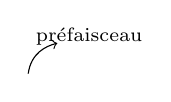
\begin{tikzpicture}[baseline=(p.base),x=1em,y=1em]\node[inner sep=0pt] (p) at (1.8,.7) {\scriptsize\uuline{pré}faisceau};\draw[->] (-.4,-.65) .. controls (-.3,.1) and (.25,.35) .. (.65,.45);\end{tikzpicture}}{\underline{\mathrm{Pr\acute epic}}}_{X'/S'}\deleted{\unsure{X/S}})=\mathrm{Pr\acute epic}(X'/S')\,
\overset{\inserted{=H1(X',\underline O_{X'}^{*})}}{\deleted{={\unsure{H^1}}(X',\underline O_{X'}^{*})=\Gamma(S',\underline H^{1}_{\unsure{X'/S'|X/S}}(\underline O^{*}_{X'}))}} & \deleted{\unsure{X}}\\[.9em]
\underline{\underline{\mathrm{Pr\acute e}\deleted{\unsure{p}}\mathrm{pic}'}}_{X/S}(S')=\Gamma(S',\underset{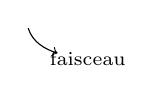
\begin{tikzpicture}[baseline=(p.base),x=1em,y=1em]\node[inner sep=0pt] (p) at (1.8,-.65) {\scriptsize faisceau};\draw[->] (-.35,.45) .. controls (-.2,-.05) and (.25,-.3) .. (.7,-.45);\end{tikzpicture}}{\underline{\mathrm{Pr\acute epic}}'}_{X'/S'})=\mathrm{Pr\acute epic}'(X'/S')\unsure{\deleted{=}|\ne|\deleted{\ne}}\quad=\Gamma(S',\underbrace{\underline H^{1}_{X'/S'}(\underline O^{*}_{X'})}_{\text{faisceau}}) & \\[.7em]
\underline{\underline{\mathrm{Pic}}}_{X/S}(S')=\Gamma(S',\underline{\mathrm{Pic}}_{X'/S'})=\mathrm{Pic}(X'/S')\quad=\widetilde{\underline{\underline{\mathrm{Pr\acute epic}}}}_{X/S}(\deleted{\unsure{X'/S'|X'}}S') & X
\end{array}\)}} 


% Lower portion: relative positions, enclosing lines, circles and hatching follow the sheet.
\figure{\resizebox{\linewidth}{!}{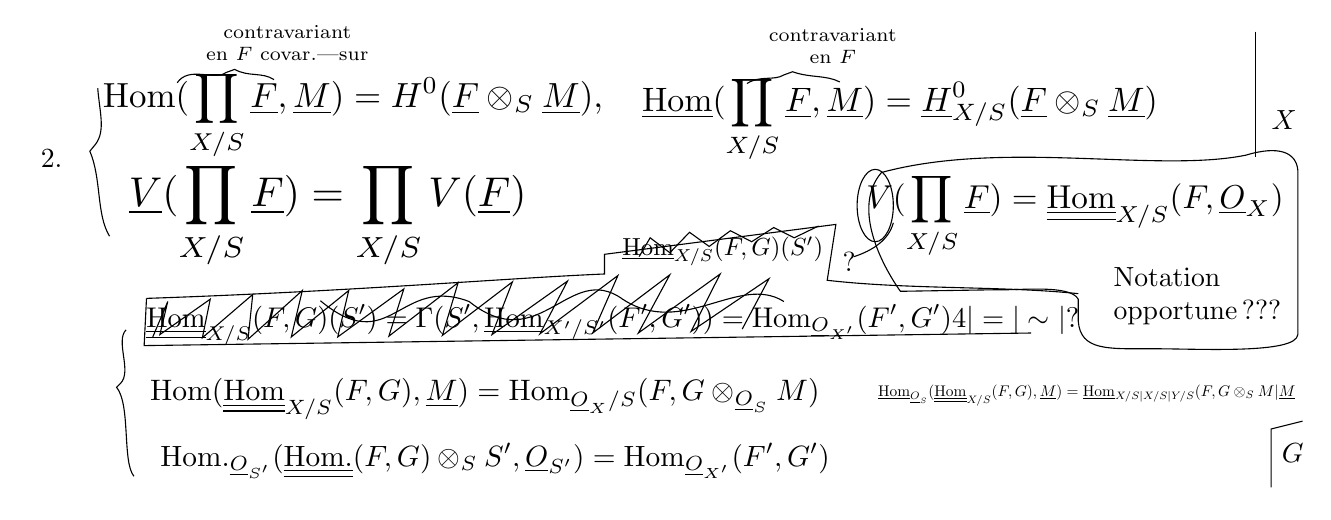
\begin{tikzpicture}[x=.01cm,y=-.01cm,every node/.style={inner sep=0pt,anchor=west}]
\useasboundingbox (0,0) rectangle (1620,590);
\node at (205,22) {\scriptsize\begin{tabular}{c}contravariant\\en $F$ \deleted{\unsure{covar.|sur}}\end{tabular}};
\node at (920,26) {\scriptsize\begin{tabular}{c}contravariant\\en $F$\end{tabular}};
\draw (190,70) .. controls (205,48) and (238,68) .. (252,57) -- (263,53) .. controls (281,63) and (298,56) .. (313,66);
\draw (914,71) .. controls (931,60) and (948,68) .. (961,60) -- (972,56) .. controls (994,64) and (1015,60) .. (1032,69);
\node at (95,112) {\resizebox{6.35cm}{!}{$\displaystyle\mathrm{Hom}(\prod_{X/S}\underline F,\underline M)=H^0(\underline F\otimes_S\underline M),$}};
\node at (780,117) {\resizebox{6.55cm}{!}{$\displaystyle\underline{\mathrm{Hom}}(\prod_{X/S}\underline F,\underline M)=\underline H^0_{X/S}(\underline F\otimes_S\underline M)$}};
\draw (1560,5)--(1560,164);\node at (1580,117) {$X$};
\node at (16,166) {$2.$};
\draw (89,77) .. controls (92,112) and (100,134) .. (83,152) -- (79,157) .. controls (94,192) and (87,237) .. (104,265);
\node at (128,239) {\resizebox{5.05cm}{!}{$\displaystyle\underline V(\prod_{X/S}\underline F)=\prod_{X/S}V(\underline F)$}};
\node at (1065,239) {\resizebox{5.30cm}{!}{$\displaystyle V(\prod_{X/S}\underline F)=\underline{\underline{\mathrm{Hom}}}_{X/S}(F,\underline O_X)$}};
\draw (1077,226) ellipse (23 and 46);
\node at (1035,298) {$?$};
\draw (1050,291) .. controls (1074,283) and (1094,270) .. (1100,248);
\draw (1085,184) .. controls (1240,142) and (1435,185) .. (1548,162) .. controls (1591,149) and (1612,159) .. (1614,181) -- (1614,390) .. controls (1612,415) and (1490,408) .. (1430,408) .. controls (1373,408) and (1338,411) .. (1335,373) -- (1335,345) .. controls (1325,326) and (1260,334) .. (1232,333) -- (1109,335) .. controls (1087,304) and (1046,229) .. (1085,184);
\node at (1358,341) {\begin{tabular}{l}Notation\\opportune\,???\end{tabular}};
\node at (755,284) {\resizebox{2.55cm}{!}{$\deleted{\underline{\mathrm{Hom}}_{X/S}(F,G)(S')}$}};
\node at (150,378) {\resizebox{11.85cm}{!}{$\displaystyle\deleted{\underline{\underline{\mathrm{Hom}}}_{X/S}(F,G)(S')=\Gamma(S',\underline{\mathrm{Hom}}_{X'/S'}(F',G'))=\mathrm{Hom}_{\underline O_{X'}}(F',G')\unsure{4|=|\sim|?}}$}};
% Stepped enclosing stroke and the broad zigzag cancellations of the abandoned definition.
\draw (151,344) .. controls (415,335) and (612,318) .. (733,313) -- (733,288) -- (1027,250) -- (1016,321) .. controls (1120,333) and (1240,328) .. (1335,338);
\draw (151,344)--(148,404)--(1275,388);
\draw (159,393)--(178,348)--(168,390)--(232,345)--(222,394)--(286,339)--(280,396)--(349,334)--(335,393)--(408,334)--(394,393)--(478,332)--(459,392)--(547,324)--(527,391)--(616,323)--(590,390)--(686,322)--(651,389)--(750,315)--(718,388)--(816,314)--(776,388)--(880,313)--(843,386)--(942,319)--(908,383);
\draw (777,291)--(791,267)--(816,286)--(841,260)--(866,278)--(893,258)--(920,272)--(948,254)--(974,267)--(1005,252);
\draw (372,347) .. controls (461,421) and (472,314) .. (561,348) .. controls (651,420) and (688,296) .. (756,345) .. controls (832,395) and (904,312) .. (961,348);
\draw (125,384) .. controls (111,398) and (133,437) .. (118,452) -- (113,457) .. controls (131,479) and (120,552) .. (135,570);
\node at (155,472) {\resizebox{8.50cm}{!}{$\displaystyle\mathrm{Hom}(\underline{\underline{\mathrm{Hom}}}_{X/S}(F,G),\underline M)=\mathrm{Hom}_{\underline O_X\deleted{\unsure{/S}}}(F,G\otimes_{\underline O_S}M)$}};
\node at (1080,467) {\resizebox{5.30cm}{!}{$\displaystyle\underline{\mathrm{Hom}}_{\underline O_S}(\underline{\underline{\mathrm{Hom}}}_{X/S}(F,G),\underline M)=\underline{\mathrm{Hom}}_{\unsure{X/S|\deleted{X/S}|Y/S}}(F,G\otimes_S\unsure{M|\underline M}$}};
\node at (168,550) {\resizebox{8.50cm}{!}{$\displaystyle\mathrm{Hom.}_{\unsure{\underline O_{S'}}}(\underline{\underline{\mathrm{Hom.}}}(F,G)\otimes_S S',\underline O_{S'})=\mathrm{Hom}_{\underline O_{X'}}(F',G')$}};
\draw (1580,584)--(1580,510)--(1620,500);\node at (1593,541) {$G$};
\end{tikzpicture}}}
% Paper watermark, sideways through the table and obscured by the writing.
\margin{\unsure{P.J.A|P.J.} \unsure{VELIN EXTRA}}
% archive sheet number: 8
